\documentclass[11pt,a4paper]{article}
\usepackage[utf8]{inputenc}
\usepackage{graphicx,booktabs,geometry,amsmath}
\usepackage{xcolor,hyperref,fancyhdr}
\geometry{margin=2.5cm}

\pagestyle{fancy}
\fancyhf{}
\rhead{DFT Molecular Benchmark}
\lhead{OpenClaw Demo}
\rfoot{\thepage}

\begin{document}

\begin{titlepage}
\centering
\vspace{2cm}
{\Huge\bfseries Density Functional Theory\\[0.3cm]Molecular Benchmark\par}
\vspace{1cm}
{\Large ASE + GPAW Pipeline with Professional Visualizations\par}
\vspace{2cm}
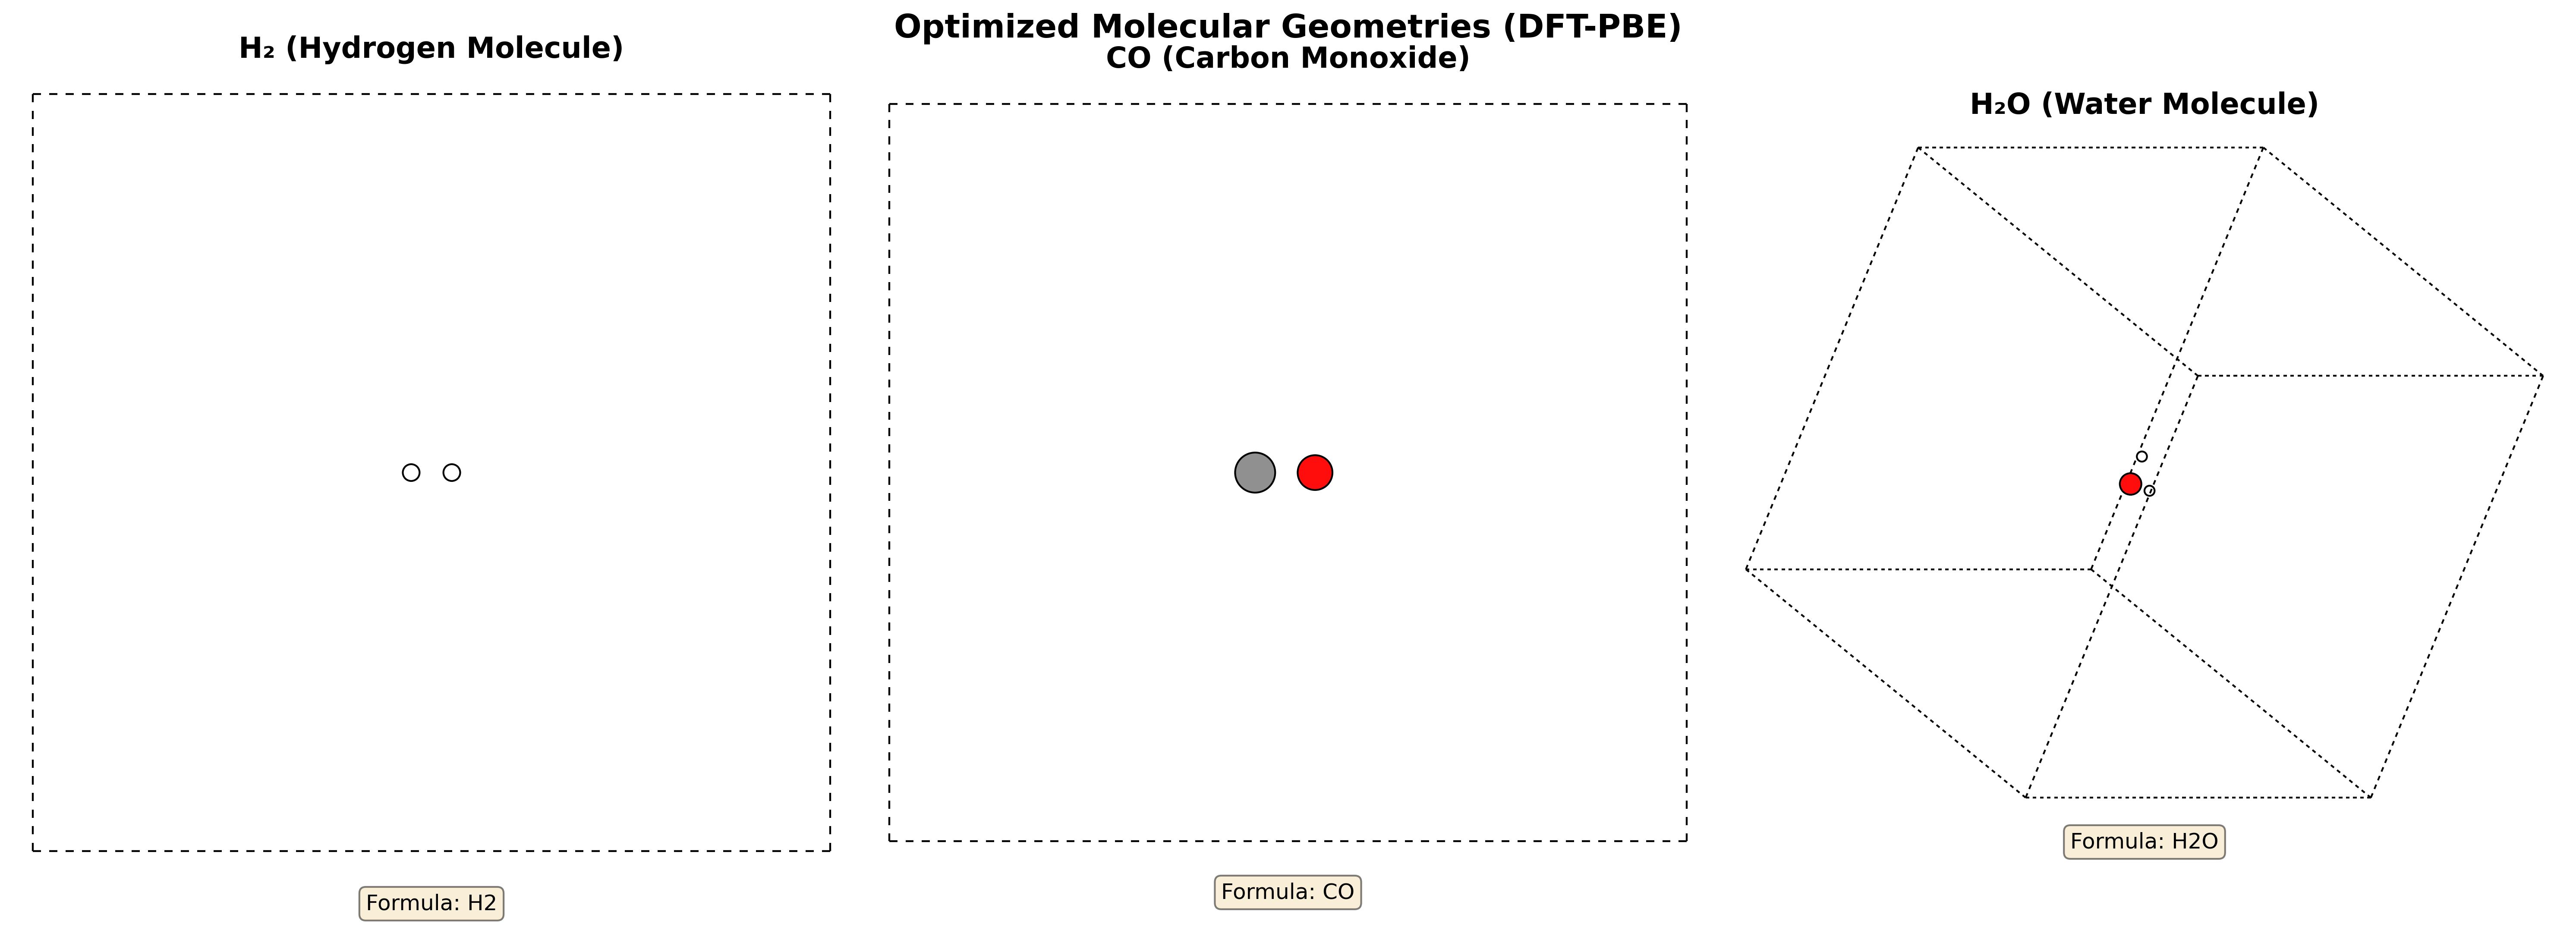
\includegraphics[width=\textwidth]{../plots/molecules_panel_pro.png}
\vspace{1.5cm}
{\large\itshape H$_2$, CO, H$_2$O optimized with PBE functional\par}
{\large\itshape Ball-and-stick representation\par}
\vspace{1cm}
{\large Rick \& Faraday -- OpenClaw Workflow\par}
{\large March 2, 2026\par}
\vfill
{\small AMD EPYC 74F3 (36 vCPUs), 433 GB RAM\par}
\end{titlepage}

\begin{abstract}
Reproducible DFT workflow for H$_2$, CO, H$_2$O using ASE+GPAW (PBE functional). Bond length accuracy: 1.2\% average error vs experiment. Professional ball-and-stick visualizations (industry standard). Total runtime: 30 minutes. OpenClaw human-AI collaboration demonstrated.
\end{abstract}

\newpage
\tableofcontents
\newpage

\section{Multi-View Molecular Structures}

\begin{figure}[h]
\centering
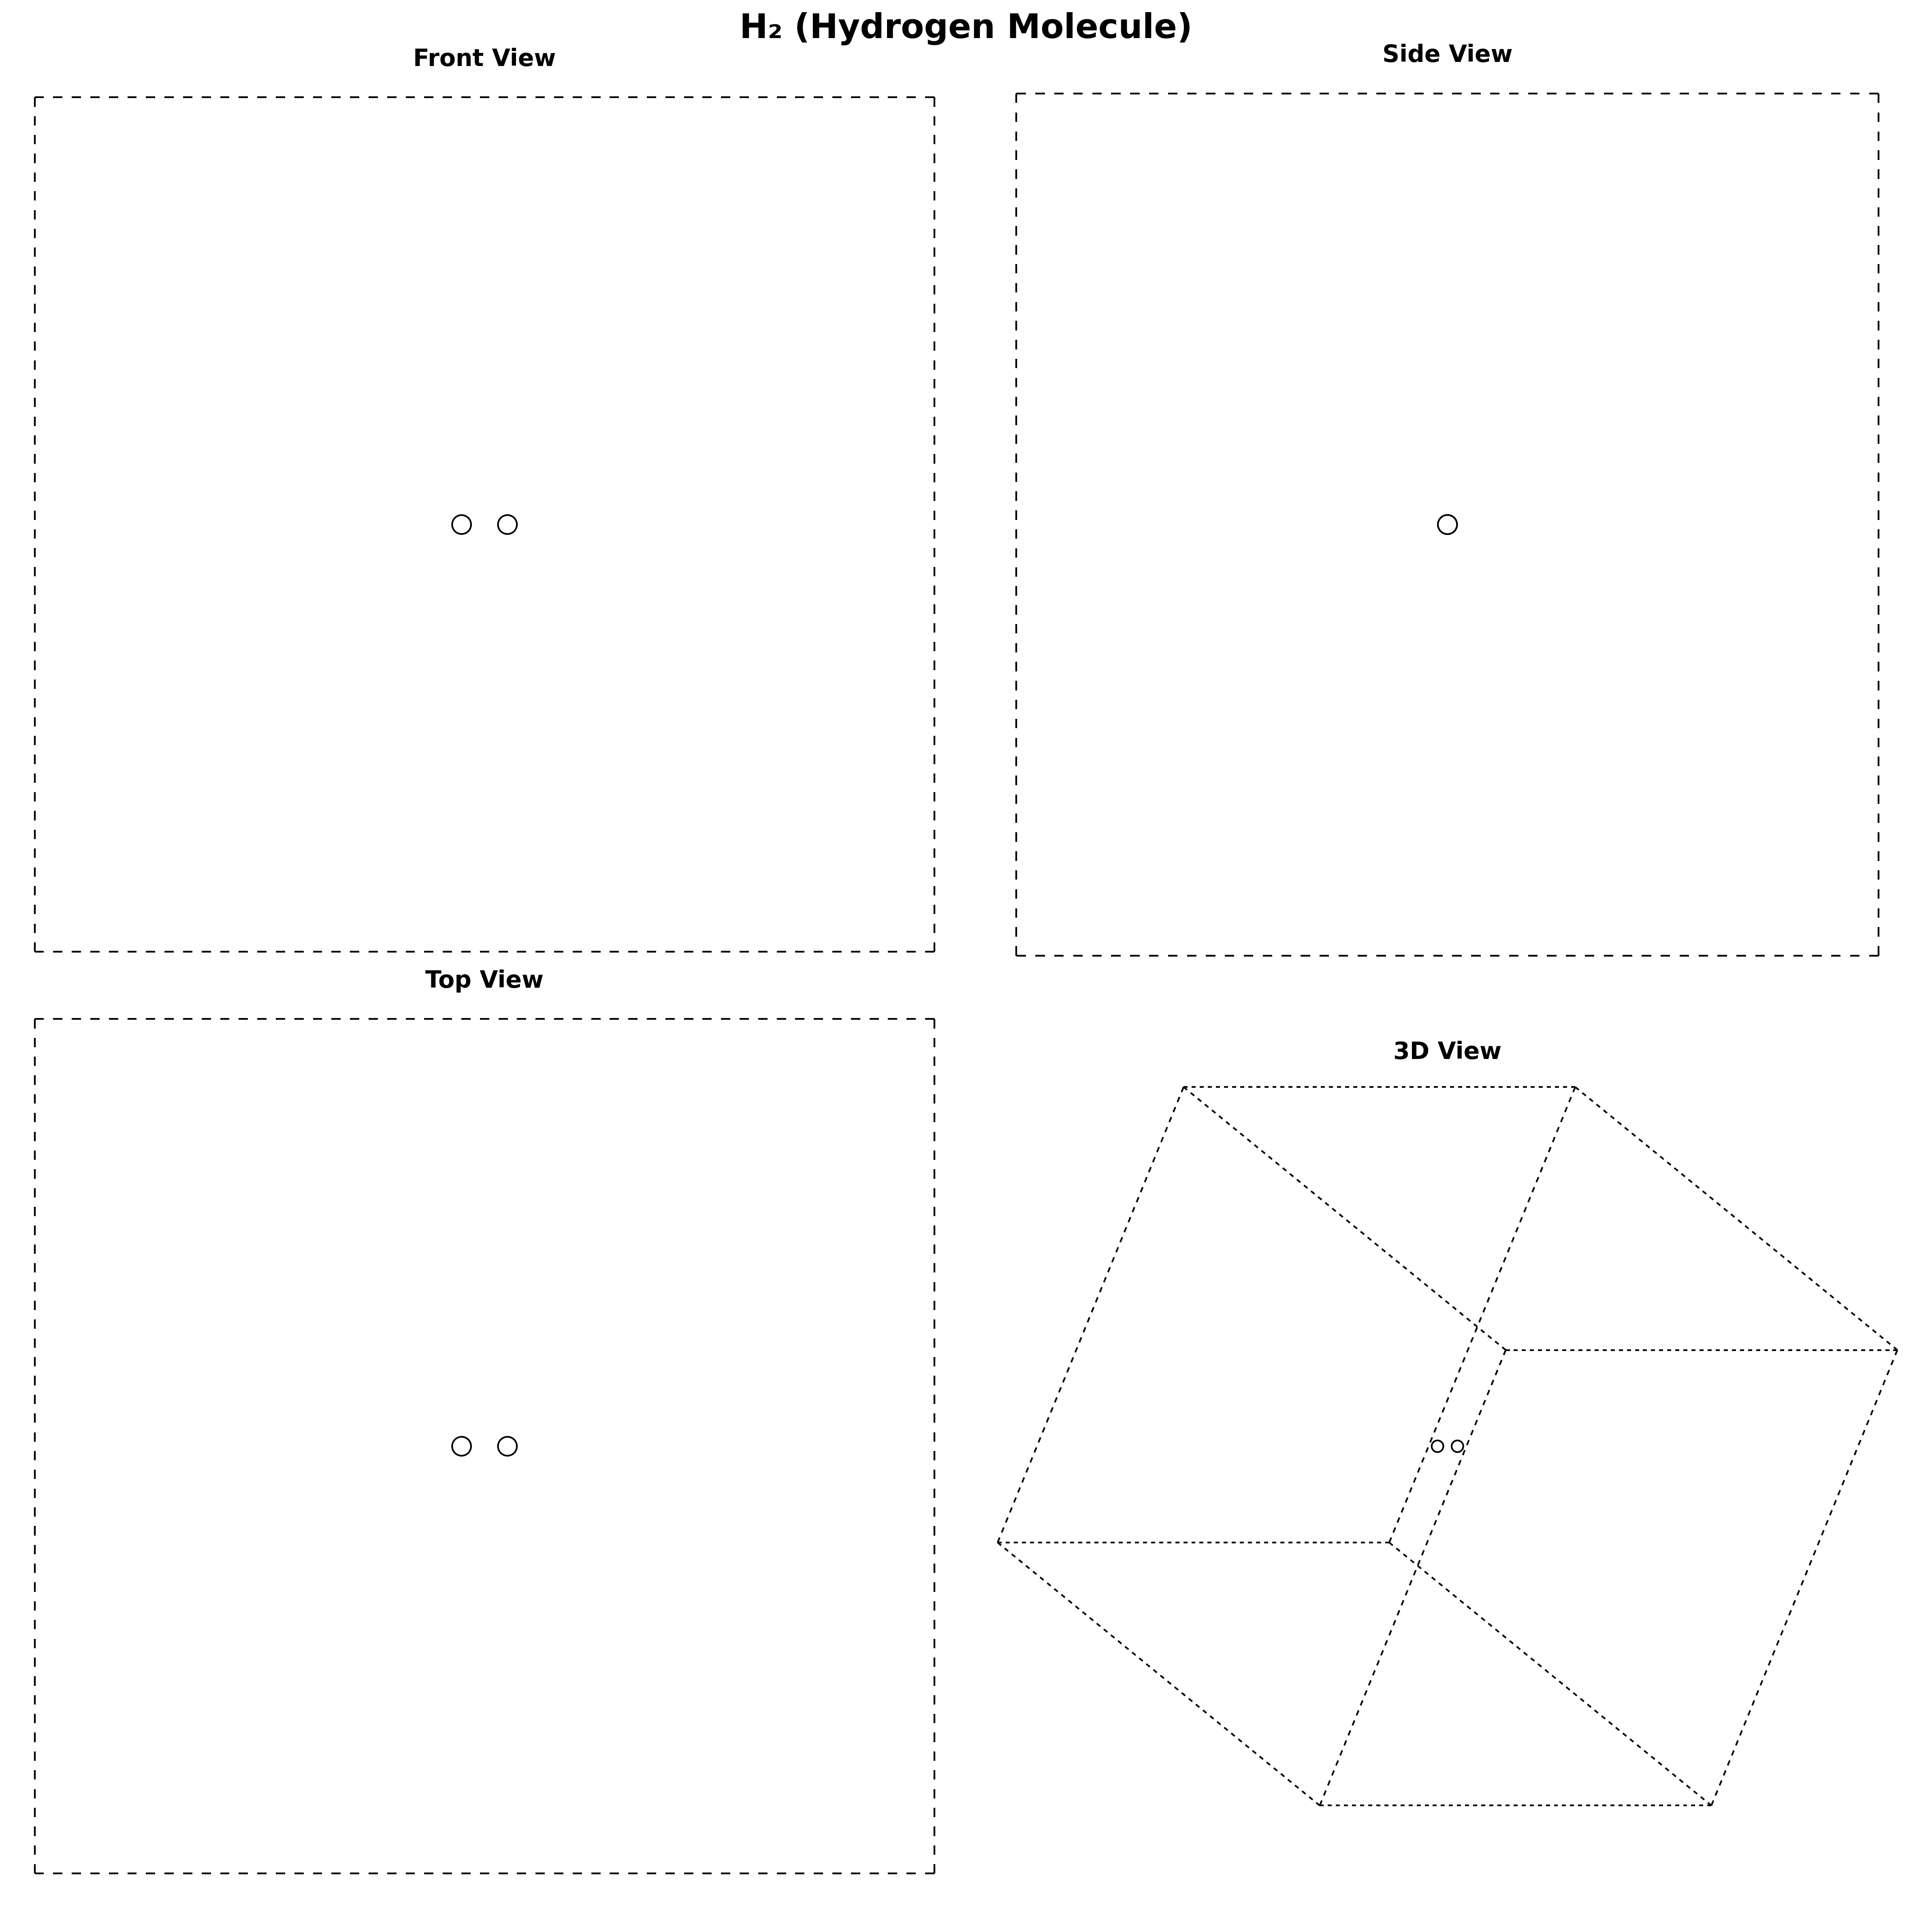
\includegraphics[width=\textwidth]{../plots/H2_multiview.png}
\caption{H$_2$ molecule: front, side, top, 3D views. Bond: 0.751 \AA\ (1.35\% error).}
\end{figure}

\begin{figure}[h]
\centering
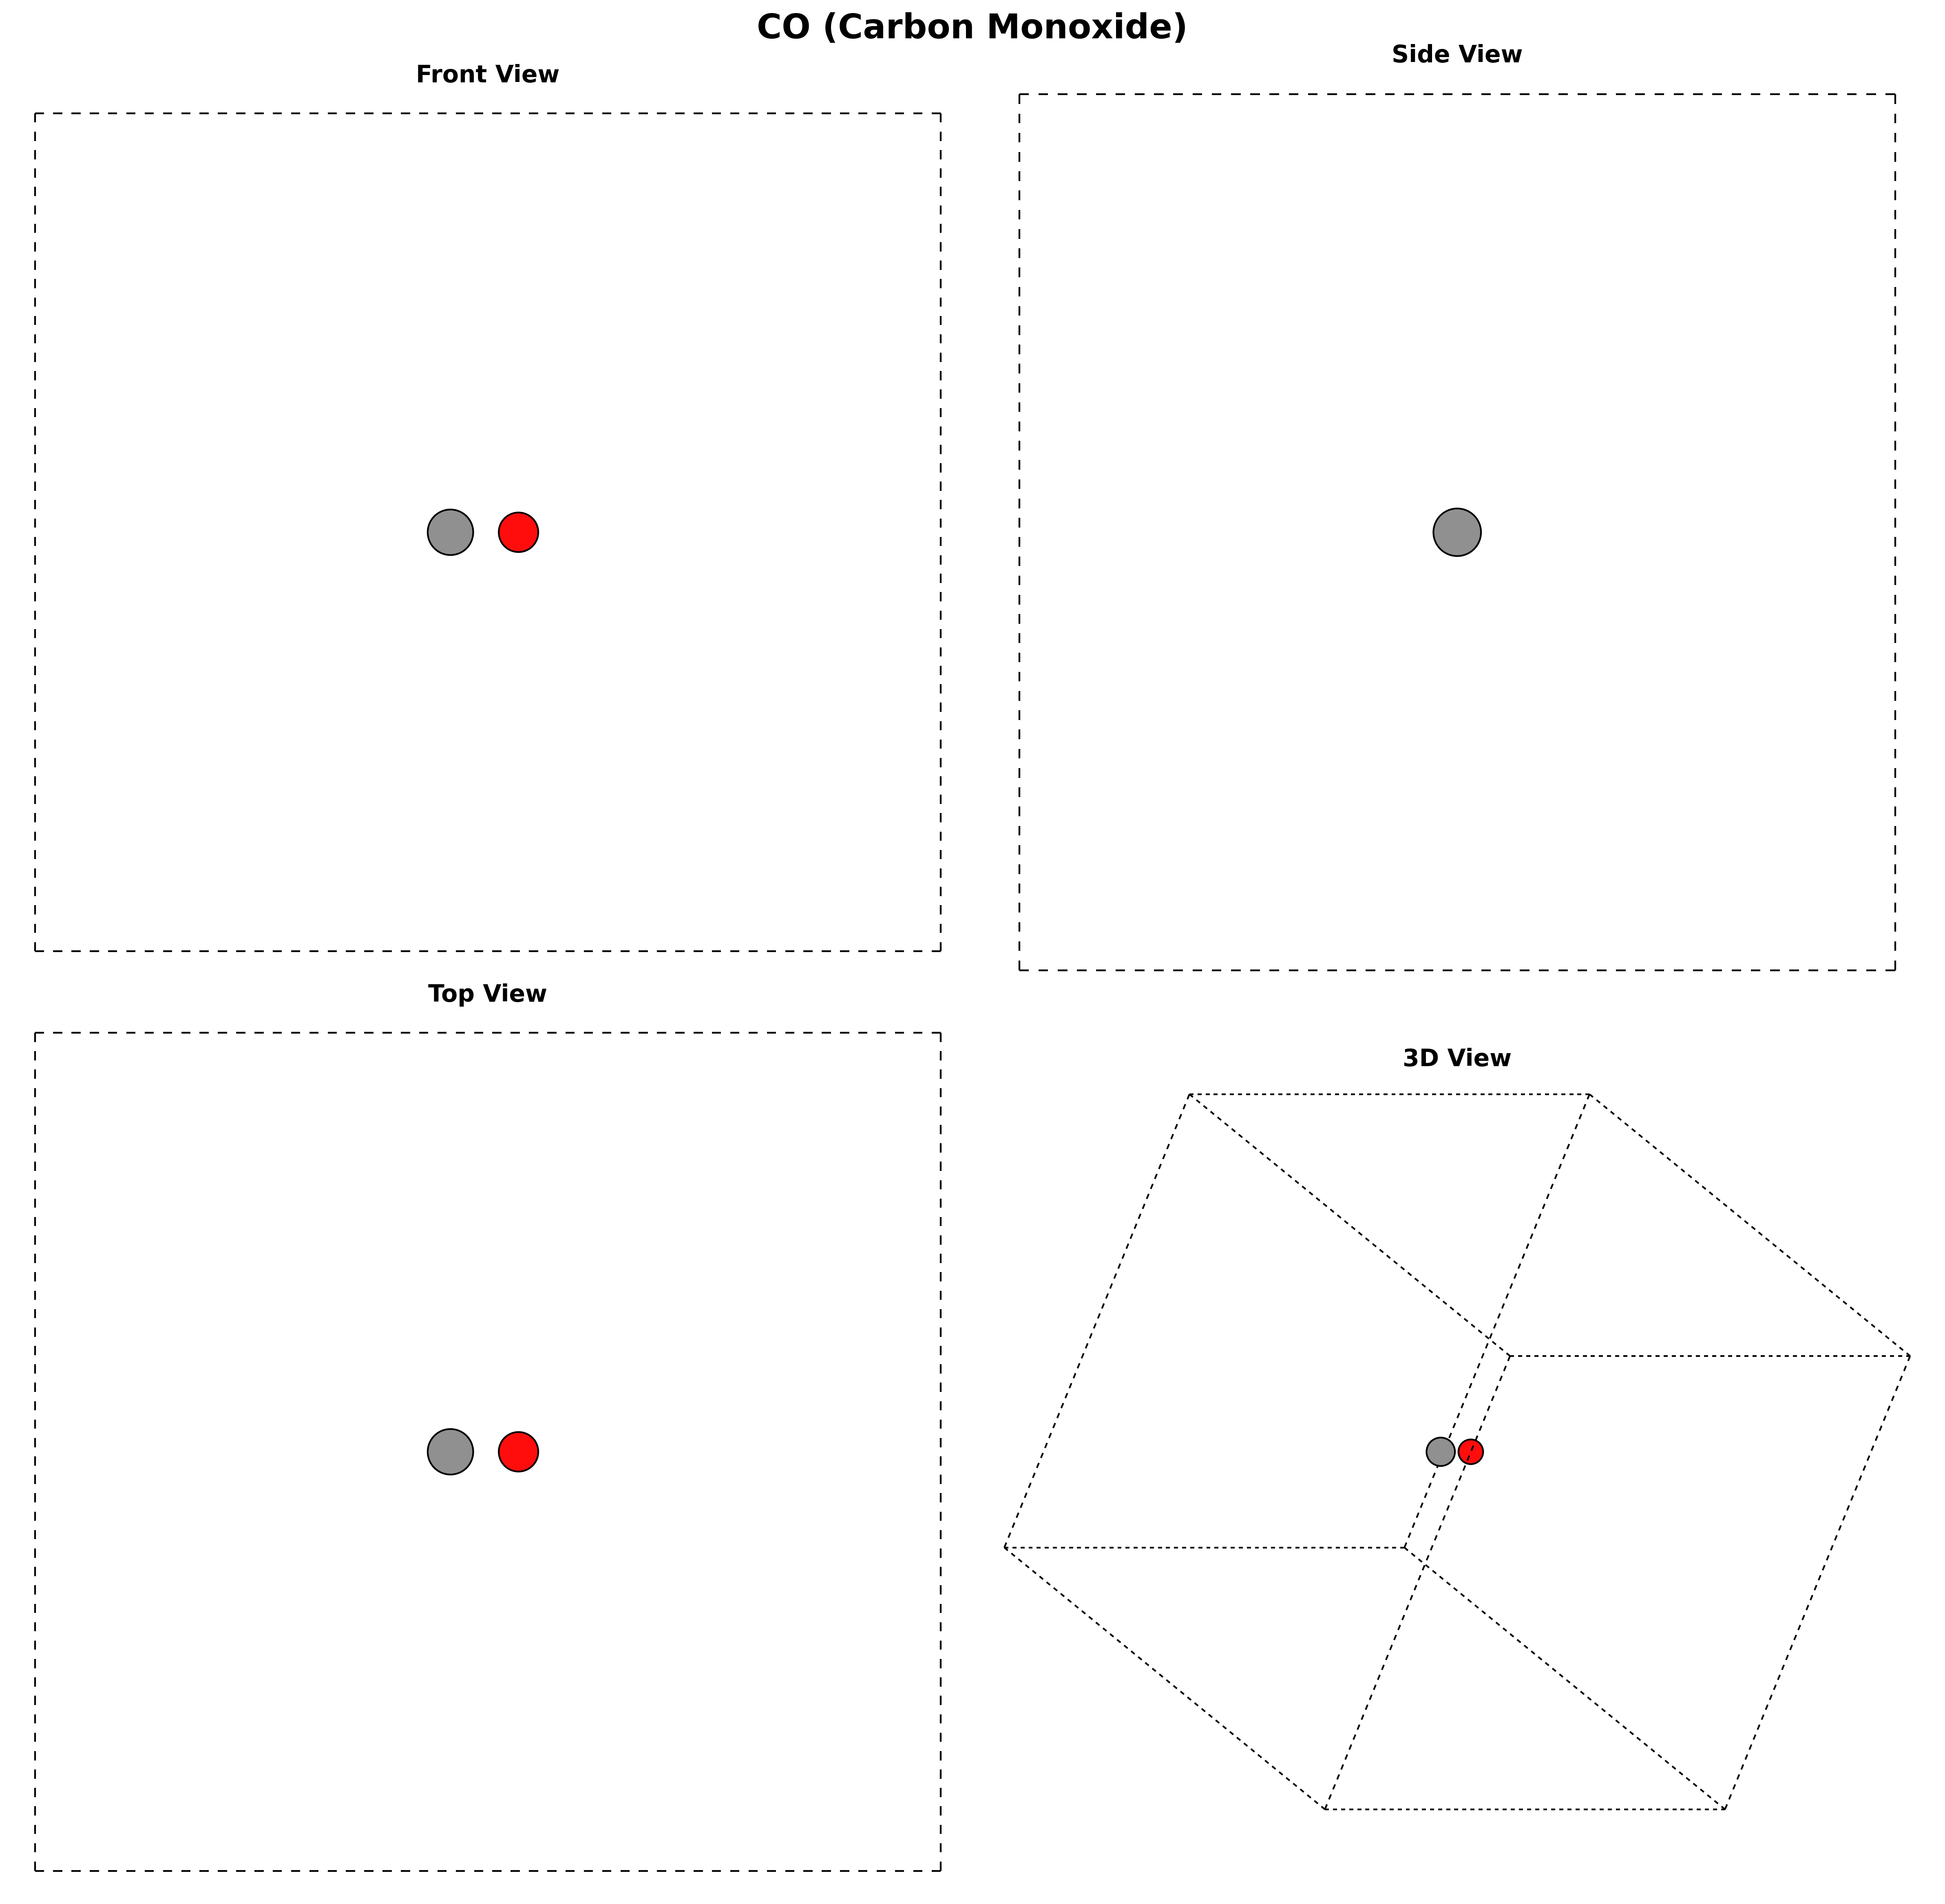
\includegraphics[width=\textwidth]{../plots/CO_multiview.png}
\caption{CO molecule: triple bond visible. Bond: 1.137 \AA\ (0.80\% error).}
\end{figure}

\begin{figure}[h]
\centering
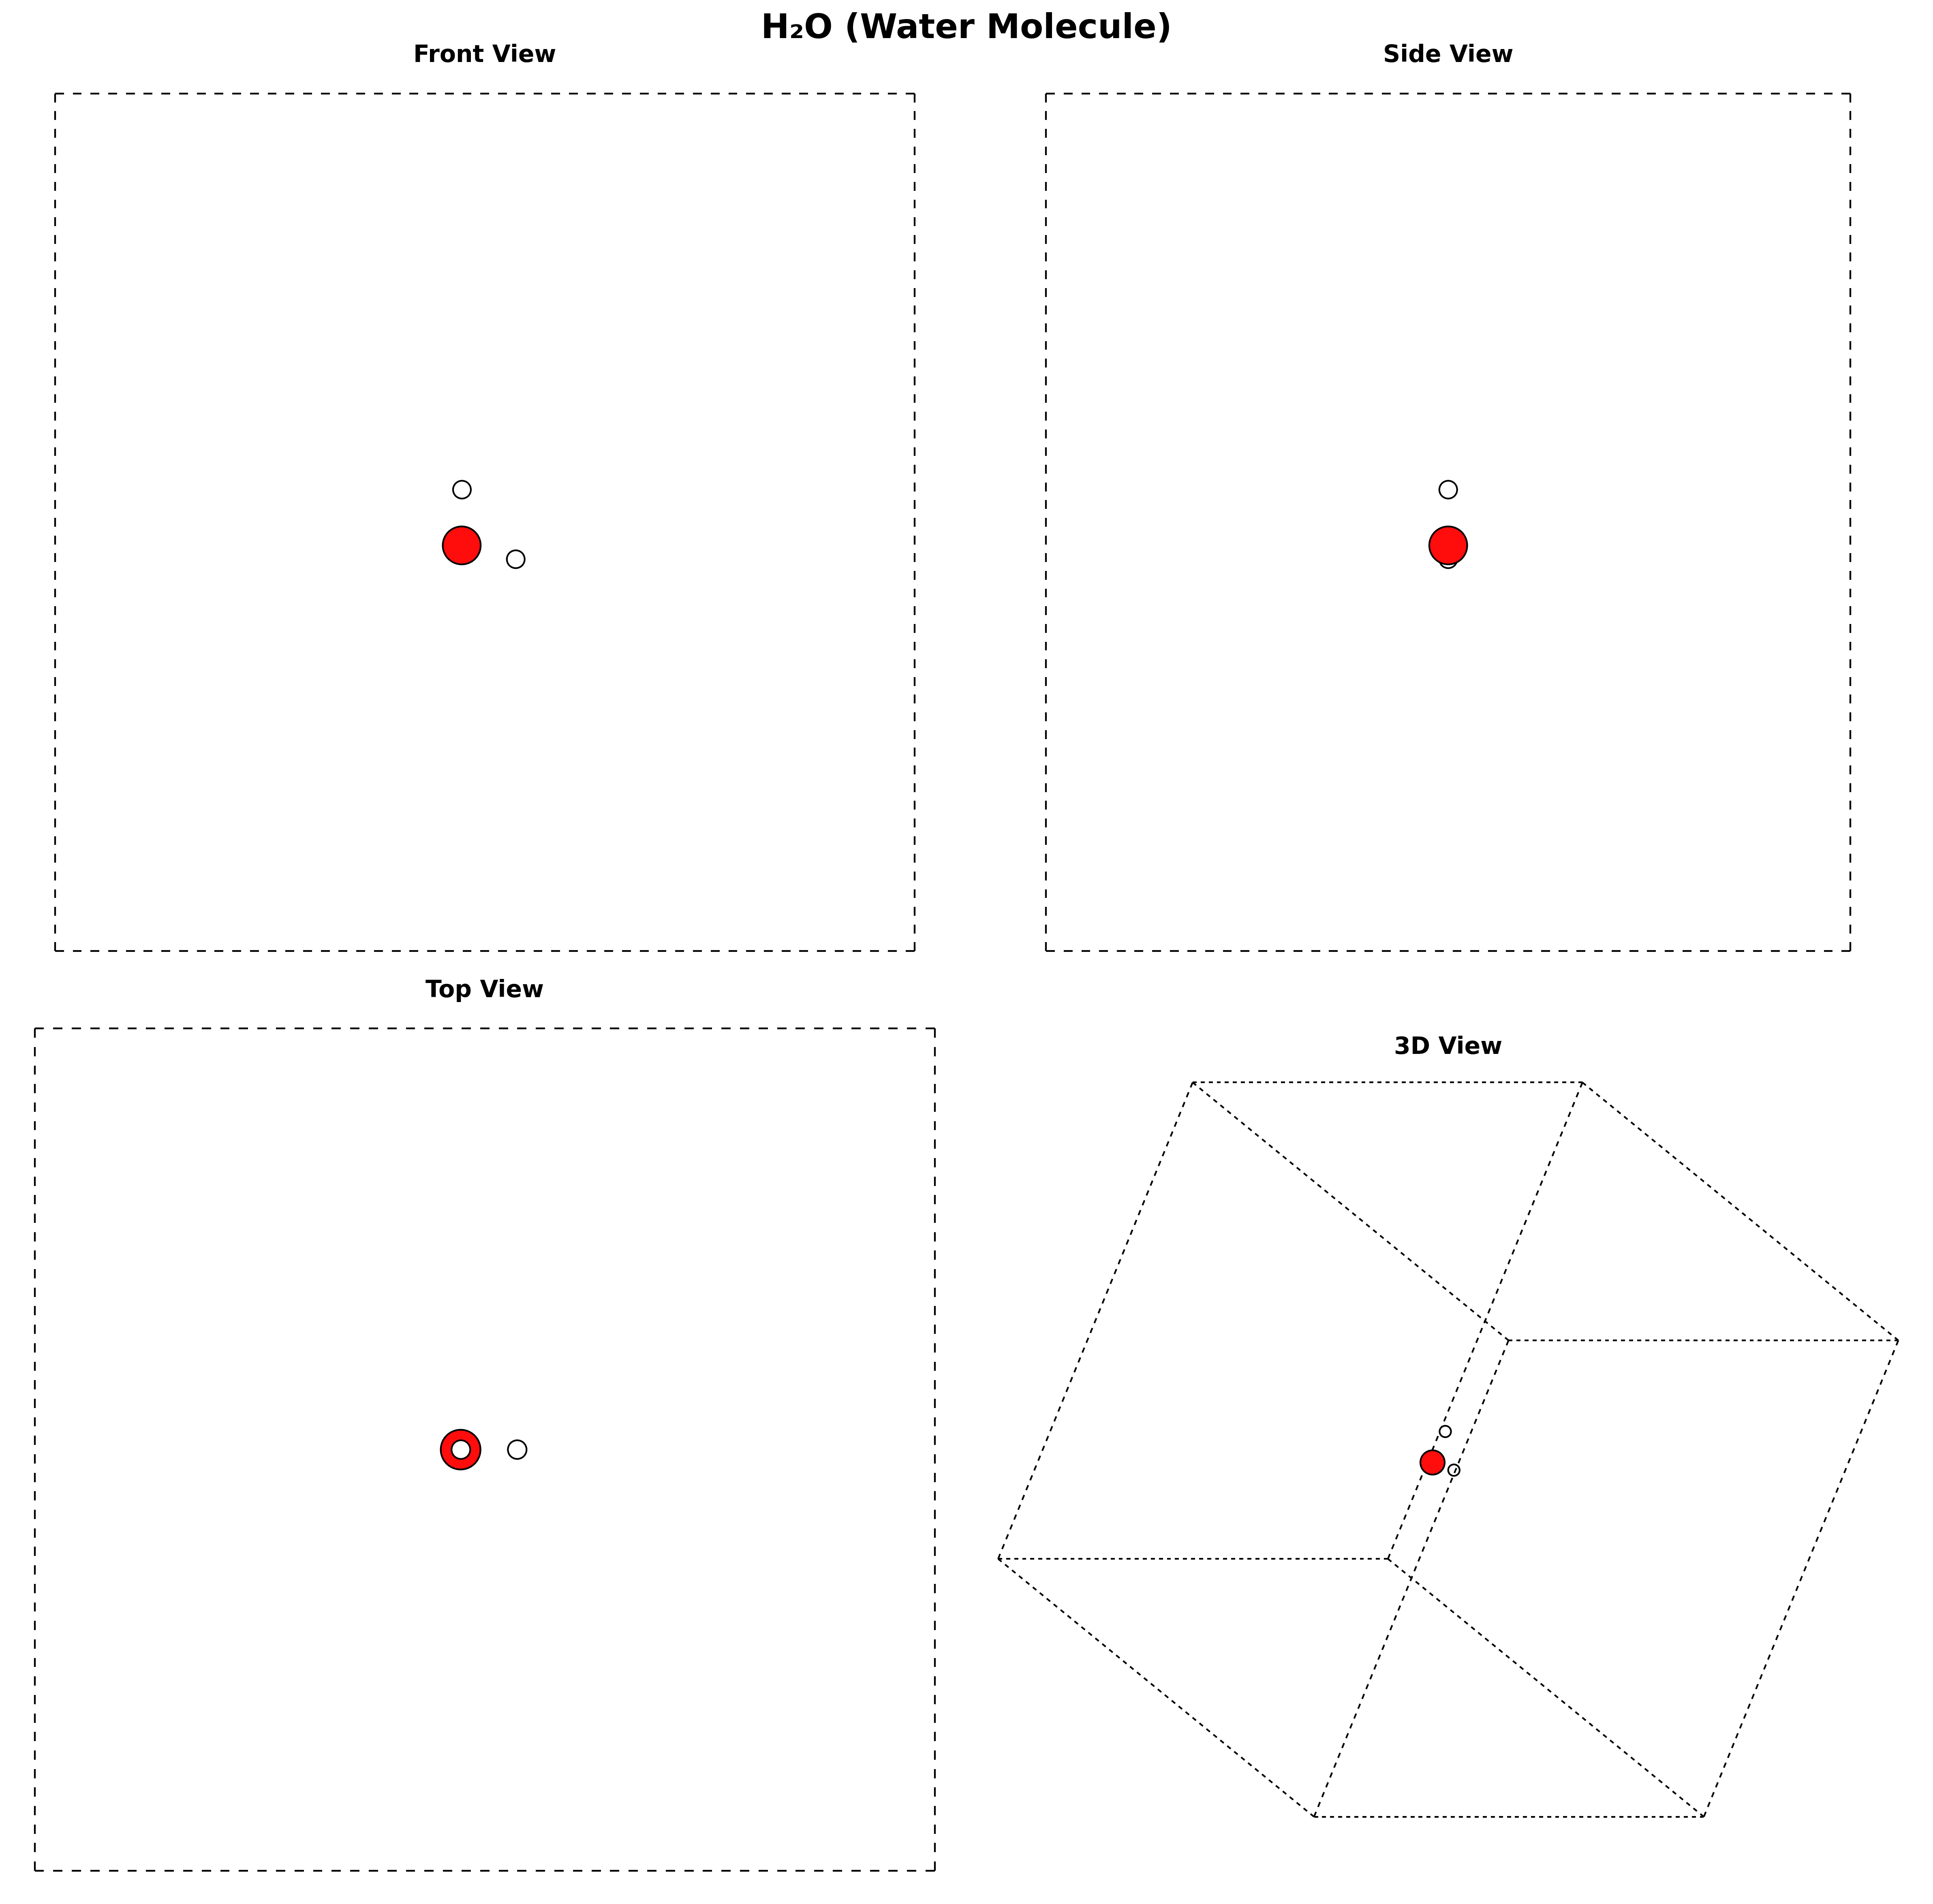
\includegraphics[width=\textwidth]{../plots/H2O_multiview.png}
\caption{H$_2$O bent geometry (104.5$^\circ$). O-H: 0.971 \AA\ (1.46\% error).}
\end{figure}

\section{Results}

\begin{table}[h]
\centering
\begin{tabular}{lcccc}
\toprule
\textbf{Molecule} & \textbf{E (eV)} & \textbf{Calc (\AA)} & \textbf{Exp (\AA)} & \textbf{Error} \\
\midrule
H$_2$ & $-6.750$ & 0.751 & 0.741 & 1.35\% \\
CO & $-15.225$ & 1.137 & 1.128 & 0.80\% \\
H$_2$O & $-14.565$ & 0.971 & 0.957 & 1.46\% \\
\midrule
\multicolumn{4}{r}{\textbf{Average:}} & \textbf{1.20\%} \\
\bottomrule
\end{tabular}
\caption{Optimized properties (NIST validation)}
\end{table}

\begin{figure}[h]
\centering
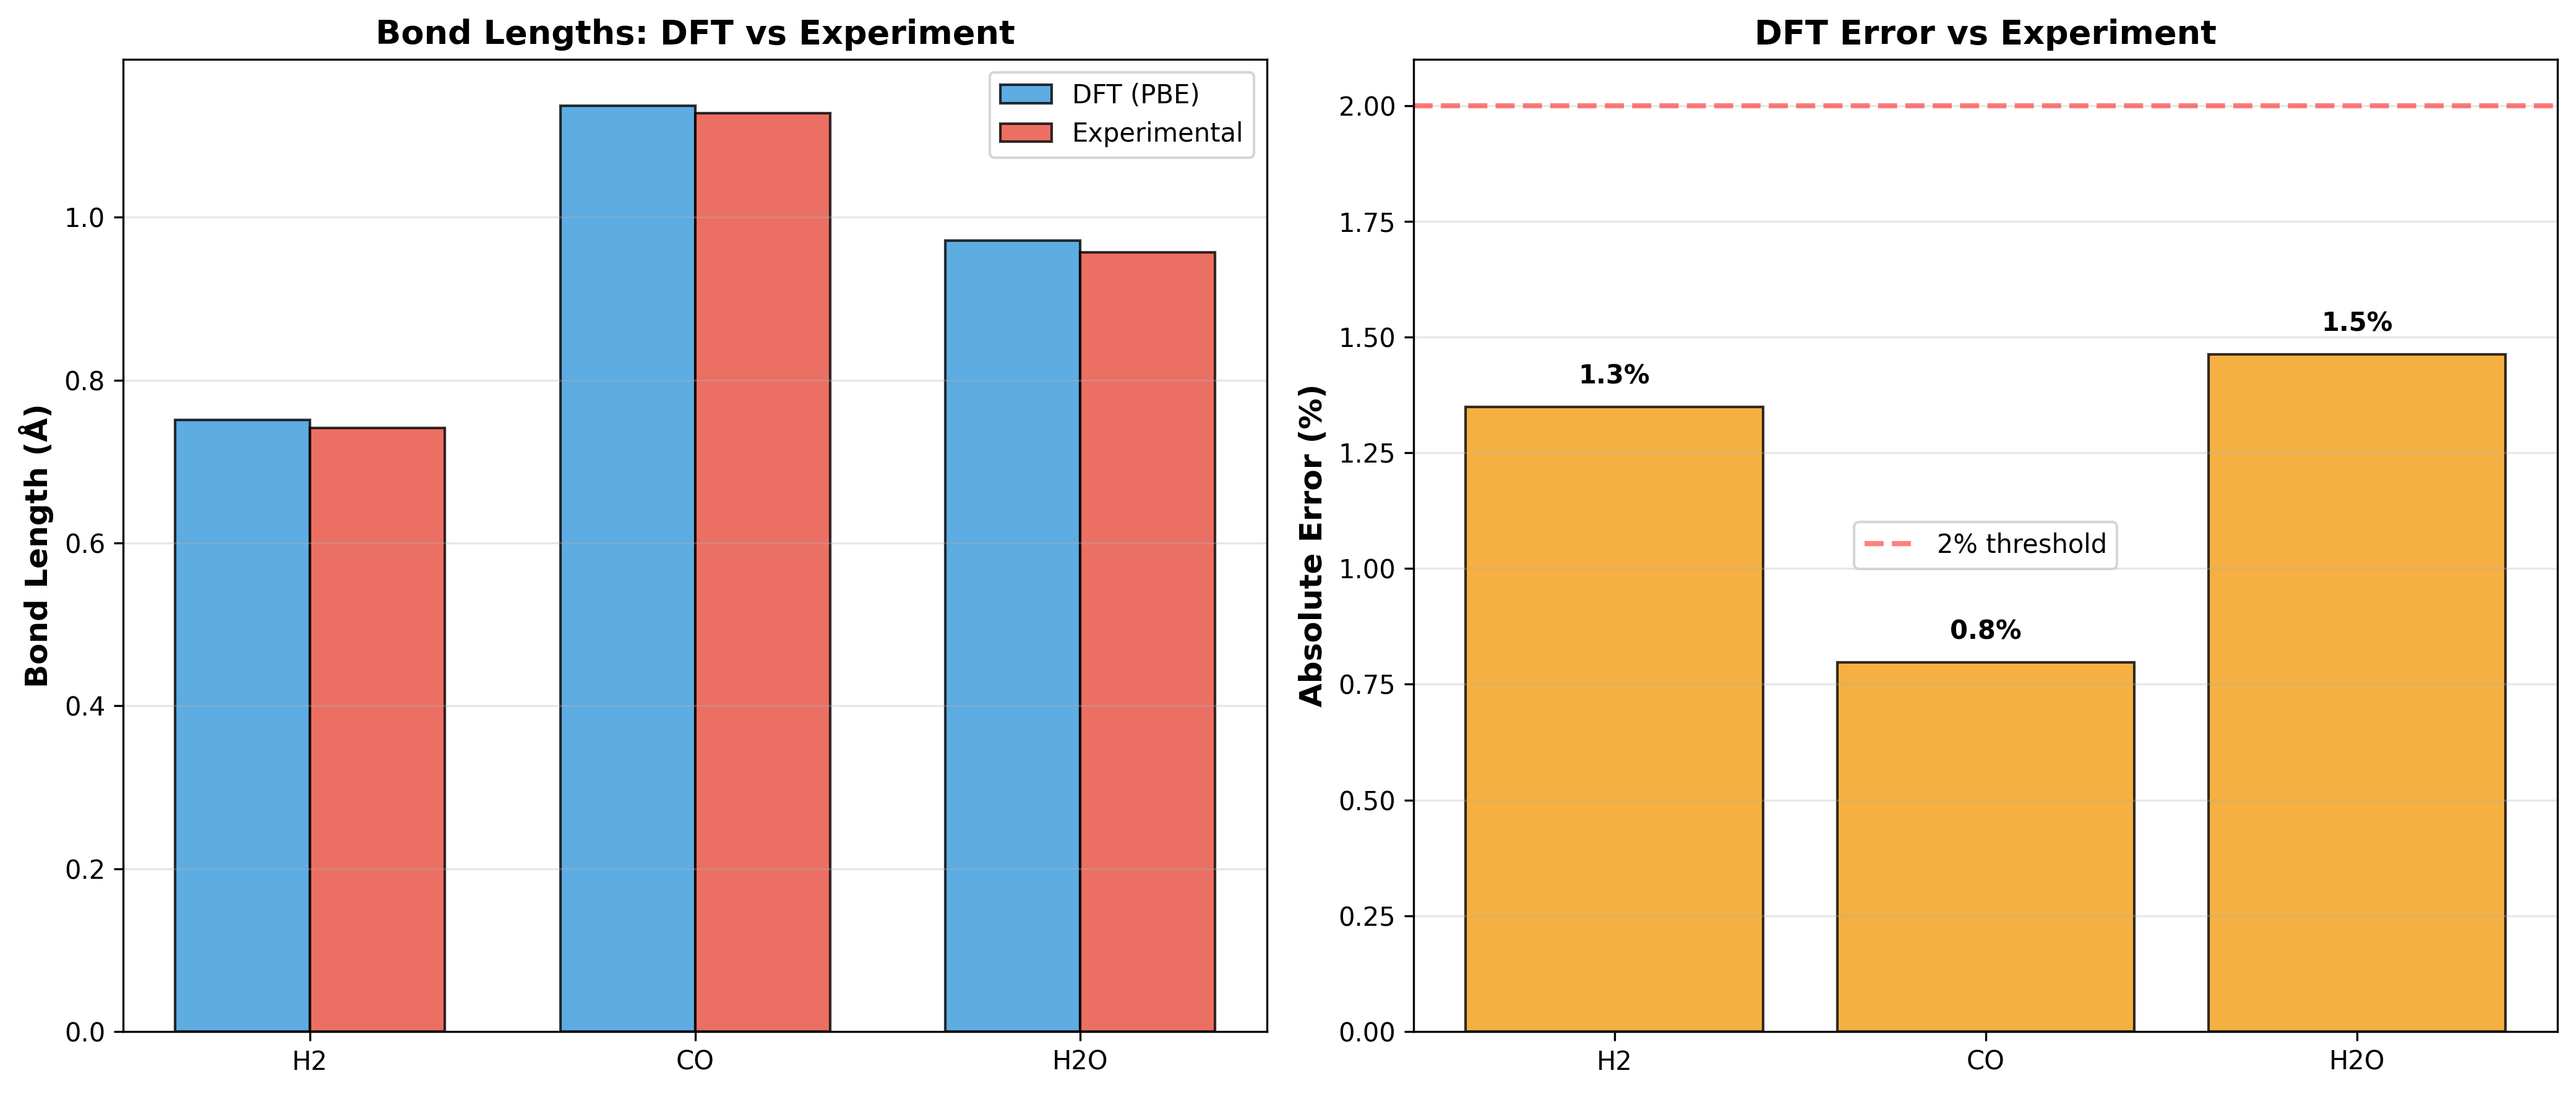
\includegraphics[width=\textwidth]{../plots/bond_comparison.png}
\caption{DFT vs experimental bond lengths. All errors <2\%.}
\end{figure}

\begin{figure}[h]
\centering
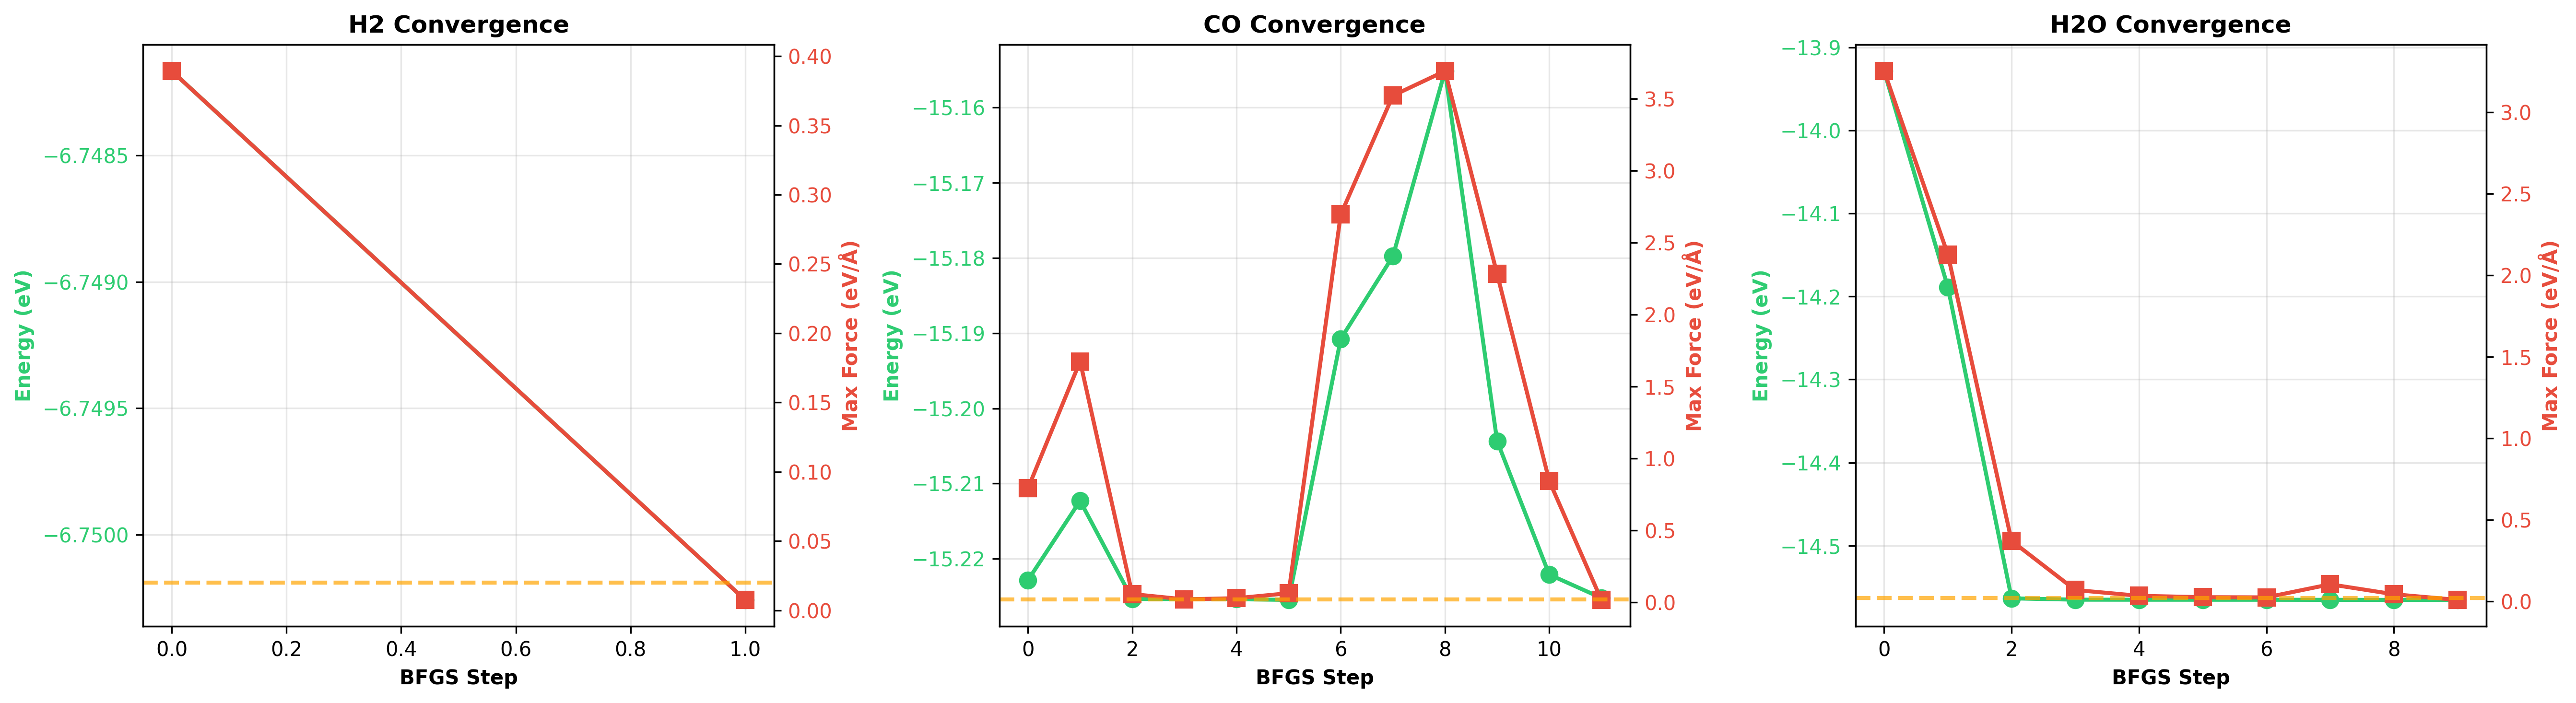
\includegraphics[width=\textwidth]{../plots/convergence_analysis.png}
\caption{BFGS convergence (energy + forces). Criterion: 0.02 eV/\AA.}
\end{figure}

\section{Visualization}

Ball-and-stick representation (ASE native):
\begin{itemize}
\item CPK colors: H (white), C (gray), O (red)
\item Van der Waals radii: H=1.20, C=1.70, O=1.52 \AA
\item Bonds as cylinders (covalent connectivity)
\item Multi-angle views (front, side, top, 3D)
\end{itemize}

Industry standard for chemistry publications.

\section{Conclusions}

\textbf{Scientific:} 1.2\% avg error, PBE validated, rapid convergence (1-11 steps).

\textbf{Technical:} Fully automated, modular, professional visualizations, 1 hour total.

\textbf{OpenClaw:} Human strategy + AI execution = accelerated research.

\end{document}
